\chapter[Permutaciones]{Permutaciones}


\begin{section}{Permutaciones}
Recordemos  que una \textit{permutación} de un conjunto finito no vacío $X$ es una biyección de $X$ en $X$. (Frecuentemente tomamos $X$ como $ [[1,n]]=\{1,2,\ldots,n\}$.) Por ejemplo una permutación típica de $[[1,5]]$ es la función $\alpha$ definida por las ecuación
$$
\alpha(1)=2,\quad \alpha(2)=4,\quad \alpha(3)=5,\quad
\alpha(4)=1,\quad \alpha(5)=3.
$$

Denotemos el conjunto de todas las permutaciones de $[[1,n]]$ con $S_n$. Por ejemplo, $S_3$ contiene las $3!=6$ permutaciones siguientes:
$$
\begin{matrix} 1&2&3 \\ \downarrow&\downarrow&\downarrow\\1 &2 &
3\end{matrix}\qquad
\begin{matrix} 1&2&3 \\ \downarrow&\downarrow&\downarrow\\1 &3 &2 \end{matrix}\qquad
\begin{matrix} 1&2&3 \\ \downarrow&\downarrow&\downarrow\\2 & 1&3 \end{matrix}
\qquad
\begin{matrix} 1&2&3 \\ \downarrow&\downarrow&\downarrow\\2 & 3&1
\end{matrix}\qquad
\begin{matrix} 1&2&3 \\
\downarrow&\downarrow&\downarrow\\3 &1 &2 \end{matrix}\qquad
\begin{matrix} 1&2&3 \\ \downarrow&\downarrow&\downarrow\\3 &2 &1
\end{matrix}
$$


En la práctica, usualmente asignamos alguna interpretación concreta a un elemento de $S_n$. Como vimos en la sección \ref{seccion-selecciones-ordenadas-sin-repeticion}, podemos usar la interpretación ``selecciones ordenadas sin repetición''  \index{selección ordenada sin repetición} donde, en este caso seleccionamos los elementos de $\{1,2,3,\ldots,n\}$ en algún orden hasta que no queda ninguno. Una interpretación relacionada es que una permutación efectúa un \textit{reacomodamiento} de $\{1,2,3,\ldots,n\}$; por ejemplo, la permutación $\alpha$ vista más arriba  efectúa el reacomodamiento de $12\,345$, en $24\,513$, así:
$$
\begin{matrix} 1&2&3&4&5 \\
\downarrow&\downarrow&\downarrow&\downarrow&\downarrow\\2 &4 &5 &1
& 3
\end{matrix}
$$
En algunas circunstancias es conveniente mirar una permutación y el correspondiente reacomodamiento como la misma cosa, pero esto puede traer dificultades si debemos considerar sucesivos reacomodamientos. Es importante tener en cuenta que 
$$
\textit{una permutación es una función con ciertas características.}
$$

Cuando las permutaciones son tratadas como funciones es claro como deben combinarse. Consideremos $\alpha$ la permutación de $[[1,5]]$ antes mencionada, y sea $\beta$ la permutación de $[[1,5]]$ dada por 
$$
\beta(1)=3,\quad \beta(2)=5,\quad \beta(3)=1,\quad
\beta(4)=4,\quad \beta(5)=2.
$$
La función compuesta $\beta\alpha$ es la permutación definida por $(\beta\alpha)(i)= \beta(\alpha(i))$ ($1\le i\le 5$), esto es 
$$
\beta\alpha(1)=5,\quad \beta\alpha(2)=4,\quad
\beta\alpha(3)=2,\quad \beta(4)\alpha=3,\quad \beta\alpha(5)=1.
$$
(Recordemos que, como siempre, $\beta\alpha$ significa ``primero $\alpha$, entonces $\beta$''.) En términos de reacomodamientos tenemos
$$\begin{aligned}
\alpha\quad&\quad\begin{matrix} 1&2&3&4&5 \\
\downarrow&\downarrow&\downarrow&\downarrow&\downarrow\\2 &4 &5 &1
& 3
\end{matrix} \\
\beta \quad&\quad \begin{matrix} 1&2&3&4&5 \\
\downarrow&\downarrow&\downarrow&\downarrow&\downarrow\\5 &4 &2 &3
& 1
\end{matrix}
 \end{aligned}
$$



Existen cuatro características de la composición de permutaciones de gran importancia, y están listadas en el próximo teorema.

\begin{teorema}\label{tA3} Las siguientes propiedades valen en el conjunto $S_n$ de todas las permutaciones de $\{1,2,3,...,n\}$.
\begin{enumerate}[label=\textit{\alph*)}]
\item  Si $\pi$ y $\sigma$ pertenecen a $S_n$, entonces $\pi\sigma$ también.
\item  Para cualesquiera permutaciones $\pi$, $\sigma$, $\tau$ en $S_n$,
$$
(\pi\sigma)\tau=\pi(\sigma\tau).$$
\item  La función identidad, denotada por $\operatorname{id}$ y definida por $\operatorname{id}(r) =r$ para todo $r$ en $\mathbb N_n$, es una permutación y para cualquier $\sigma$ en $S_n$,
tenemos
$$
\operatorname{id}\sigma=\sigma\operatorname{id}=\sigma.$$
\item  Para toda permutación $\pi$ en $S_n$ hay una permutación inversa $\pi^{-1}$ en $S_n$ tal que
$$
\pi\pi^{-1} = \pi^{-1}\pi = \operatorname{id}.
$$
\end{enumerate}
\end{teorema}
\begin{proof} Todas las afirmaciones se deducen de propiedades conocidas de funciones en general y funciones biyectivas en particular. Por otro lado, es fácil convencerse de la validez de las mismas mirando las permutaciones como reacomodamiento de elementos. 
\end{proof}


Es conveniente tener una notación más compacta para las permutaciones. Consideremos otra vez la permutación $\alpha$ de $\{1,2,3,4,5\}$, y notemos en particular que
$$
\alpha(1)=2,\qquad \alpha(2)=4,\qquad \alpha(4)=1.
$$
Así $\alpha$ lleva $1$ a $2$, $2$ a $4$ y $4$ a $1$, y por esta razón decimos que los símbolos $1, 2, 4$ forma un \textit{ciclo } (de longitud $3$). Del mismo modo, los símbolos $3$ y $5$ forman un ciclo de longitud $2$, y
escribimos:
$$
\alpha=(1\,2\,4)(3\,5).
$$
Esta es la \textit{notación cíclica} para $\alpha$. Cualquier \index{notación cíclica} permutación $\pi$ puede ser escrita cíclicamente de la siguiente manera:
\begin{itemize}
\item comencemos con algún símbolo (digamos el $1$) y veamos el efecto de $\pi$ sobre él y sus sucesores hasta que alcancemos el $1$
nuevamente;
\item elijamos un símbolo que todavía no haya aparecido y construyamos el ciclo que se deriva de él; 
\item repitamos el procedimiento hasta que se terminen los símbolos.
\end{itemize}
Por ejemplo, la permutación $\beta$ definida antes tiene la notación cíclica
$$
\beta=(1\,3)(2\,5)(4),
$$
donde observamos que el símbolo $4$ forma un ciclo ``degenerado'' por sí solo, puesto que $\beta(4)=4$. En algunas ocasiones podemos omitir estos ciclos de longitud 1 cuando escribimos una permutación en notación cíclica, puesto que corresponden a símbolos que no son afectados por la permutación. Sin embargo, usualmente es útil \textit{no} adoptar esta convención hasta que uno se familiariza con la notación.


Aunque la representación de una permutación en notación cíclica es esencialmente única, hay dos manera obvias en las que podemos cambiar la notación sin alterar la permutación. Primero, cada ciclo puede empezar en cualquiera de sus símbolos; por ejemplo $(7\,8\,2\,1\,3)$ y $(1\,2\,7\,8\,2)$ describen el mismo ciclo. Segundo, el orden de los ciclos no es importante; por ejemplo $(1\,2\,4) (3\,5)$ y $(3\,5) (1\,2\,4)$ denotan la misma permutación. Pero las características importantes son el número de ciclos, la longitud del ciclo, y la disposición de los símbolos dentro de los ciclos, y éstas están determinadas de manera única. Por eso, la rotación cíclica nos dice bastantes cosas útiles sobre una permutación.

\begin{ejemplo}\label{cartas} Cartas numeradas del $1$ al $12$ son distribuidas en una mesa en la manera en que se muestra en la parte izquierda de la tabla que sigue. Luego las cartas son levantadas  por filas (de izquierda a derecha y de arriba hacia abajo) y se redistribuyen con el mismo arreglo, pero por columnas, no por filas (de arriba hacia abajo y de izquierda a derecha), apareciendo como se muestra en la parte derecha de la tabla.
$$
\begin{matrix} 1& 2& 3\\
4 &5 &6 \\
7 &8 & 9\\
10 &11 & 12 \end{matrix}\qquad \qquad\qquad
\begin{matrix}1 &5 &9 \\
2 &6 &10 \\
3& 7& 11\\
4&8 & 12 \end{matrix}
$$
¿Cuántas veces debe repetirse este procedimiento hasta que las cortas aparezcan dispuestas como estaban inicialmente?
\end{ejemplo}
\begin{proof}[Solución] Sea $\pi$ la permutación que efectúa el reordenamiento; esto es $\pi(i) =j$ si la carta $j$ aparece en la posición previamente ocupada por la carta $i$. Trabajando con la notación cíclica para $\pi$ encontramos que
$$
\pi=(1)(2\,\,5\,\,6\,\,10\,\,4)(3\,\,9\,\,11\,\,8\,\,7)(12).
$$
Los ciclos degenerados $(1)$ y $(12)$ indican que las cartas 1 y 12 nunca cambian de posición. Las otros ciclos tienen longitud 5, así que cuando el proceso se haya realizado 5 veces las cartas
reaparecerán en sus posiciones originales. Otra forma de expresar el resultado es decir que $\pi^5= \operatorname{id}$, donde $\pi^5$ representa las cinco repeticiones de la permutación $\pi$.
\end{proof}
\end{section}


\subsection*{$\S$ Ejercicios}
\begin{enumex}
\item Escribir en notación cíclica la permutación que realiza el siguiente reordenamiento:
$$
\begin{matrix} 1&2&3&4&5&6&7&8&9 \\
\downarrow&\downarrow&\downarrow&\downarrow&
\downarrow&\downarrow&\downarrow&\downarrow&\downarrow
\\ 3&5 &7 &8 &4 &6 &1 &2 &9
\end{matrix}
$$

\item Sean $\sigma$ y $\tau$ las permutaciones de $[[1,8]]$ cuyas representaciones en la notación cíclica son
$$
\sigma= (1\,2\,3)(4\,5\,6)(7\,8),\qquad
\tau=(1\,3\,5\,7)(2\,6)(4)(8).
$$
Escribir en notación cíclica $\sigma\tau$, $\tau\sigma$, $\sigma^2$, $\sigma^{-1}$, $\tau^{-1}$. 

\item Resolver el problema presentado en el ejemplo \ref{cartas} cuando hay $20$ cartas acomodadas en $5$ filas de $4$.

\item Probar que hay exactamente tres elementos de $S_4$ que tienen dos ciclos de longitud $2$, escritos en la notación cíclica. 

\item Sea $K$ el subconjunto de $S_4$ que contiene la identidad y las tres permutaciones descritas en el ejercicio previo. Escribir la ``tabla de multiplicación'' para $K$, interpretando la multiplicación como la composición de permutaciones.

\item Calcular en número total de permutaciones $\sigma$ de $\mathbb [[1,6]]$ que satisfacen $\sigma^2=\text{id}$ y $\sigma\not=\text{id}$.
\item Sean $\alpha$ y $\beta$ permutaciones de $[[1,9]]$ cuyas representaciones en la notación cíclica son:
$$
\alpha= (1237)(49)(58)(6),\qquad \beta=(135)(246)(789).
$$
Escribir en notación cíclica $\alpha\beta$, $\beta\alpha$, $\alpha^2$, $\beta^2$, $\alpha^{-1}$, $\beta^{-1}$.

\item Sea $X_1=\{0,1\}$, y para $i\ge 2$ definamos $X_i$ como el conjunto de subconjuntos de $X_{i-1}$. Encontrar el valor más pequeño para el cual $|X_i|>10^{100}$.

\item Por cada entero $i$ en el rango $1 \le i \le n-1$ definimos $\tau_i$ como la permutación de $[[1,n]]$ que intercambia $i$ e $i+1$ y no afecta los otros elementos. Explícitamente 
$$
\tau_i = (1)(2)\cdots(i-1)(i\ i+1)(i+2)\cdots(n).
$$
Probar que toda permutación de $[[1,n]]$ puede ser expresada en términos de $\tau_1,\tau_2,\ldots,\tau_{n-1}$. 

\item Una permutación de $[[1,n]]$ que tenga solo un ciclo (necesariamente de longitud $n$) es llamada \textit{cíclica}  \index{permutación cíclica}. Probar que hay $(n-1)!$ permutaciones cíclicas de $[[1,n]]$.

\item Un mazo de $52$ cartas es dividido en dos partes iguales y luego se alternan las cartas de una y otra parte. Es decir si la numeración original era $1,2,3,\ldots,54$, el nuevo orden es $1,27,2,28,\ldots$ ¿Cuántas veces se debe repetir este procedimiento para obtener de nuevo el mazo original? 
\end{enumex}


\chapter[El principio del tamiz]{El principio del tamiz} \label{ape.principio_del_tamiz}

\begin{section}{El principio del tamiz}\label{Ap1.2}
El principio más básico del conteo (proposición \ref{principiodeadicion}) dice que $|A \cup B|$ es la suma de $|A|$ y $|B|$, cuando $A$ y $B$ son conjuntos disjuntos. Si $A$ y $B$ no son disjuntos, cuando sumamos $|A|$ y $|B|$ estamos contando $A \cap B$ dos veces. Entonces, para obtener la respuesta correcta debemos restar $|A \cap B|$:
$$
|A \cup B| = |A|+|B| - |A \cap B|.
$$

Un método similar puede aplicarse a tres conjuntos. Cuando sumamos $|A|$, $|B|$ y $|C|$, los elementos de $A \cap B$, $B \cap C$, y $C \cap A$ son contados dos veces (si no están en los tres conjuntos). Para corregir esto, restamos $|A \cap B|$, $|B \cap C|$ y $|C \cap A|$. Pero ahora los elementos de $A \cap B \cap C$, contados originalmente tres veces, han sido descontados tres veces. Luego, para conseguir la respuesta correcta, debemos sumar $|A \cap B \cap C|$. Así
$$
|A \cup B\cup C|= \alpha_1-\alpha_2+\alpha_3,
$$ 
donde
$$\gathered
\alpha_1=|A|+|B|+|C|,\qquad \alpha_2= |A \cap B|+|B \cap C|+|C \cap A|, \\
\alpha_3 = |A \cap B \cap C|.
\endgathered
$$

Este resultado es un caso simple de lo que suele ser llamado, por razones obvias, el principio de inclusión y exclusión. También \index{principio de inclusion y exclusion} se lo llama el \textit{principio del tamiz}.  \index{principio del tamiz}

\begin{teorema}\label{tA1.2} Si $A_1,A_2,\ldots,A_n$ son conjuntos finitos, entonces 
$$ |A_1 \cup A_2 \cup \ldots \cup A_n|= \alpha_1-\alpha_2+\alpha_3 + \cdots +(-1)^n\alpha_n, $$ donde $\alpha_i$ es la suma de los cardinales de las intersecciones de los conjuntos tomados de a $i$ por vez ($1\le i \le n$).
\end{teorema}
\begin{proof} Debemos demostrar que cada elemento $x$ de la unión hace una contribución neta de 1 al miembro de la derecha. Supongamos que $x$ pertenece a $k$ de los conjuntos $A_1, A_z,\ldots,A_n$. Entonces $x$  contribuye con $k$ en la suma $\alpha_1=|A_1|+\cdots+|A_n|$. En la suma $\alpha_2$, $x$ contribuye 1 en $|A_i \cap A_j|$ cuando $A_i$ y $A_j$ están entre los $k$ conjuntos que contienen a $x$. Existen $\binom{k}{2}$ de esos pares, por lo tanto $\binom{k}{2}$ es la contribución de $x$ a $\alpha_2$. En general la contribución de $x$ a $\alpha_i$ ($1 \le i \le n$) es $\binom{k}{i}$. Por lo tanto el total con que contribuye $x$ al lado derecho de la igualdad es 
$$
\binom{k}{1} -\binom{k}{2} + \cdots + (-1)^{k-1} \binom{k}{k},
$$
porque los términos con $i > k$ dan cero.

Por el teorema del binomio aplicado a $(1-1)^k=0$, se deduce que la expresión de arriba  es igual a
$\binom{k}{0}$, que vale $1$.
\end{proof}

Un corolario simple del teorema \ref{tA1.2} es a menudo más útil en la práctica. Supongamos que $X$ es un conjuntos finito y $A_1,A_2,\ldots,A_n$ son subconjuntos de $X$ (cuya unión no necesariamente es igual a $X$). Si $|X| = N$, entonces el número de elementos de $X$ que no están en ninguno de esos subconjuntos es
$$\begin{aligned}
|X-(A_1 \cup A_2 \cup \ldots \cup A_n)|&=
|X|-|A_1 \cup A_2 \cup \ldots \cup A_n| \\
&= N- \alpha_1 + \alpha_2 - \cdots + (-1)^n\alpha_n.
\end{aligned}
$$

\begin{ejemplo*} Hay $73$ estudiantes en el primer año de la Escuela de Artes de la universidad. De ellos, $52$ saben tocar el piano, $25$ el violín y $20$ la flauta; $17$ pueden tocar tanto el piano como el violín, $12$ el piano y la flauta; pero solo Juan Rictero puede tocar los tres instrumentos ¿Cuántos alumnos no saben tocar ninguno de esos instrumentos?
\end{ejemplo*}
\begin{proof}[Solución] Con $V$, $P$ y $F$ denotaremos los conjuntos de estudiantes que saben tocar el violín, el piano y la flauta respectivamente. Usando la información dada tenemos que $$
\begin{aligned}
\alpha_1&= |P| + |V| + |F|= 52+25+20=97 \\
\alpha_2&= |P\cap V| + |V\cap F| + |P\cap F|=17+7+12=36 \\
\alpha_3&= |P\cap V\cap F|= 1.
\end{aligned}
$$
Por consiguiente, el número de estudiantes que o pertenecen a ninguno de los tres conjuntos $P$, $V$ y $F$ es
$$
73-97+36-1=11.
$$
\end{proof}

\begin{ejemplo*} Una secretaria ineficiente tiene $n$ cartas distintas y $n$ sobres con direcciones ¿De cuántas maneras puede ella arreglárselas para meter cada carta en un sobre equivocado? (Esto es comúnmente llamado el \textit{problema del desarreglo} del cual hay varias formulaciones pintorescas.) 
\end{ejemplo*}


\begin{proof}[Solución] Podemos considerar cada carta y su correspondiente sobre  como si estuvieran etiquetadas con un entero $i$ en el rango $1 \le i \le n$. El acto de poner las cartas en los sobres puede describirse como una permutación $\pi$  de $\mathbb N_n$: $\pi(i)=j$ si la carta $i$ va en el sobre $j$. Necesitamos saber  el número de \textit{desarreglos}, esto es, las permutaciones $\pi$ tales que
$\pi(i)\not=i$ para todo $i$ en $\mathbb N_n$.

Denotemos $A_i$ ($1 \le i \le n$) el subconjunto de $S_n$ (el conjunto de permutaciones de $\mathbb N_n$) que contiene aquellos $\pi$ tales que $\pi(i)=i$. Diremos que los elementos de $A_i$ \textit{fijan} $i$. Por el principio del tamiz, el número de desarreglos es 
$$
d_n= n! -\alpha_1+\alpha_2 - \cdots +(-1)^n\alpha_n,
$$
donde $\alpha_r$ es la suma de los cardinales de las intersecciones de los $A_i$ tomando r por vez. En otras palabras, $\alpha_r$ es el número de permutaciones que fijan $r$ símbolos dados, tomando todas las maneras de elegir los $r$ símbolos. Ahora hay $\binom{n}{r} $ maneras de elegir $r$ símbolos, y el número de  permutaciones que los fijan es solo el número de permutaciones de los restantes $n-r$ símbolos, que es $(n-r)!$  Por lo tanto
$$
\alpha_r = \binom{n}{r} \cdot (n-r)! = \frac{n!}{r!},\qquad d_n=
n!\left(1-\frac{1}{1!} + \frac{1}{2!}-\cdots
+(-1)^n\frac{1}{n!}\right). \nopagebreak$$
\end{proof}

\subsection*{$\S$ Ejercicios}
\begin{enumex}
\item En una clase de $67$ estudiantes de matemática, $47$ leen francés, $35$ leen alemán y $23$ leen ambos lenguajes ¿Cuántos estudiantes no lee ninguno de los dos lenguajes? Si además $20$ leen ruso, de los
cuales $12$ también leen francés, $11$ leen alemán y $5$ leen los tres lenguajes, ¿cuántos estudiantes no leen ninguno de los tres lenguajes?

\item Encontrar el número de formas de ordenar las letras A, E, M, O, U, Y en una secuencia de tal forma que las palabras ME e YOU no aparezcan. 

\item
Calcular el número $d_4$ de desarreglos de $\{1,2,3,4\}$ y escriba, en la notación cíclica, las permutaciones relevantes.

\item Usar el principio de inducción para probar que la fórmula para $d_n$ satisface la recursión
$$
d_1=0, \quad d_2=1,\quad d_n= (n-1)(d_{n-1}+d_{n-2}) \ (n\ge 3).
$$

\item Probar que el número de desarreglos de $\{1,2,\ldots,n\}$ en el cual un objeto dado (digamos el $1$) está en un $2$-ciclo es $(n-1)d_{n-2}$. Utilizar esto para dar una prueba directa de la fórmula recursiva del ejercicio anterior.
\end{enumex}

\end{section}


\chapter[La función de Euler]{La función de Euler}\label{ape.funcion_de_euler}

 \begin{section}{La función de Euler} \label{A2.1 }

 En esta sección probaremos un útil e importante teorema, usando sólo  los conceptos de conteo más básicos.

 El teorema se refiere a las  propiedades de divisibilidad de los enteros. Recordemos que dos enteros $x$ e
 $y$ son \textit{coprimos} si el $\mcd(x,y) = 1$. Por cada $n \ge 1$ sea  $\phi(n)$ el número de  enteros $x$ en el rango $1 \le x \le n$ tal que $x$ y $n$ son coprimos.  Podemos  calcular los primeros valores de $\phi(n)$ haciendo una tabla (tabla  \ref{tablaA2.1.1}).

La función es llamada \textit{función de Euler}, debido a Leonhard Euler  \index{Euler, Leonhard} ($1\,707-1\,783$). Cuando $n$ es primo, digamos $n=p$, cada uno de los enteros $1,2,\ldots,p-1$ es coprimo con $p$, entonces tenemos 
$$
\phi(p)=p-1,\qquad\text{ $p$ primo.}
$$

\begin{table}[h]
\begin{center}
       \begin{tabular}{r|r|r}
              $n$&  Coprimos a $n$ \,&\,$\phi(n)$\\
             \hline
              $1$&$1$&$1$ \\
              $2$&$1$&$1$ \\
              $3$&$1$,$2$&$2$ \\
              $4$&$1$,$3$&$2$ \\
              $5$&$1$,$2$,$3$,$4$&$4$ \\
              $6$&$1$,$5$&$2$ \\
              $7$&$1$,$2$,$3$,$4$,$5$,$6$&$6$ \\
              $8$&$1$,$3$,$5$,$7$&$4$
       \end{tabular}
\end{center}
 \caption{Primeros valores de $\phi(n)$} \label{tablaA2.1.1}
\end{table}

Nuestra tarea ahora es probar un resultado respecto a la suma de los valores $\phi(d)$, donde los $d$ son todos los divisores de un número positivo $n$ dado. Por ejemplo, cuando $n=12$, lo divisores $d$ son $1$, $2$, $3$, $4$, $5$, $6$ y $12$, podemos ver que
\begin{align*}
&\quad\phi(1)+\phi(2)+\phi(3)+\phi(4)+\phi(6)+\phi(12)\\
&= 1 +1+2+2+2+4 \\
&=12.
\end{align*}

Debemos demostrar que la suma es siempre igual al entero $n$ dado.

\begin{teorema}\label{tA2.1b} Para cualquier $n$ entero positivo,
$$
\sum_{d|n} \phi(d)=n.
$$
\end{teorema}
\begin{proof} Sea $S$ el conjunto de pares de enteros $(d,f)$ que
satisfacen
$$
d|n, \qquad 1\le f \le d, \qquad \mcd(f,d)=1.
$$


\begin{table}
\begin{tabular}{rr|rrrrrrrrrrrrr|c}
  &$f$ &$1$  &$2$ &$3$ &$4$ &$5$  &$6$ &$7$ &$8$ &$9$ &$10$ &$11$ &$12$ & &$\phi(d)$\\
$d$ &  &   &  &  &  &   &  &  &  &  &   &   &   & &   \\\hline
$1$ &  &$12$ &  &  &  &   &  &  &  &  &   &   &   & &$1$  \\
$2$ &  &$6$  &  &  &  &   &  &  &  &  &   &   &   & &$1$  \\
$3$ &  &$4$  &$8$ &  &  &   &  &  &  &  &   &   &   & &$2$  \\
$4$ &  &$3$  &  &$9$ &  &   &  &  &  &  &   &   &   & &$2$  \\
$6$ &  &$2$  &  &  &  &$10$ &  &  &  &  &   &   &   & &$2$  \\
$12$&  &$1$  &  &  &  &$5$  &  &$7$ &  &  &   &$11$ &   & &$4$  \\
  &  &   &  &  &  &   &  &  &  &  &   &   &   & &$12$
\end{tabular}
\caption{} \label{tablaA2.1.2}
\end{table}


La tabla \ref{tablaA2.1.2} muestra $S$ cuando $n=12$; la ``marca'' que indica que $(d,f)$ pertenece a $S$ es un número cuya importancia explicaremos en seguida. Por lo general, el número de ``marcas'' en la fila $d$ es el número de $f$'s en el rango $1\le f\le d$ que satisfacen que el $\mcd(d,f)=1$; esto es $\phi(d)$. Por lo tanto, contando $S$ por el método de las filas obtenemos
$$
|S| = \sum_{d|n} \phi(d).
$$
Para demostrar que $|S|=n$ debemos construir una biyección $\beta$ de $S$ en $\mathbb N_n$. Dado un par $(d,f)$ en $S$, definimos
$$
\beta(d,f) = f n/d.
$$
En la tabla, $\beta(d,f)$ es la ``marca'' en la fila $d$ y la columna $f$. Como $d| n$, el valor de $\beta$, es un entero y como $1\le f\le d$, entonces $\beta(d,f)$ pertenece a $\mathbb N_n$.

Para probar que $\beta$ es una inyección observemos que
$$
\beta(d,f) = \beta(d',f') \quad \Rightarrow \quad fn/d = f'n/d'
\quad \Rightarrow \quad fd'=f'd.
$$
Pero $f$ y $d$ son coprimos, así como también lo son $f'$ y $d'$, así que podemos concluir que $d=d'$ y $f=f'$.

Para demostrar que $\beta$ es una suryección, supongamos que nos dan un $x$ que pertenece a $\mathbb N_n$. Sea $g_x$ el mcd de $x$ y $n$, y sea
$$
d_x = n/g_x, \qquad f_x = x /g_x.
$$
Puesto que $g_x$ es un divisor de $x$ y $n$, entonces $d_x$ y $f_x$ son enteros, y como $g_x$ es el mcd, $d_x$ y $f_x$ son coprimos. Ahora
$$
\beta(d_x,f_x) = f_x n/d_x = x,
$$
y por lo tanto $\beta$ es suryectiva.  Luego $\beta$ es biyectiva y $|S|=n$, como queríamos demostrar.
\end{proof}

\subsection*{$\S$ Ejercicios}
\begin{enumex}
\item Encontrar los valores de $\phi(19),\quad \phi(20),\quad \phi(21)$.

\item Probar que si $x$ y $n$ son coprimos, entonces lo son $n-x$ y $n$. Deducir que $\phi(n)$ es par para todo $n \ge 3$.

\item Probar que, si $p$ es un primo y $m$ es un entero positivo, entonces un entero $x$ en el rango $1 \le x \le p^m$ \textit{no} es coprimo a $p^m$ si y solo si es un múltiplo de $p$. Deducir que $\phi(p^m) = p^m - p^{m-1}$.

\item Encontrar un contraejemplo que confirme que es falsa la conjetura $\phi(ab)= \phi(a)\phi(b)$, para enteros cualesquiera $a$ y $b$. Trate de modificar la conjetura de tal forma que no pueda
encontrar un contraejemplo. 

\item Probar que para cualesquiera enteros positivos $n$ y $m$ se cumple: 
$$
\phi(n^m) =n^{m-1}\phi(n).
$$

\item Calcular $\phi(1\,000)$ y $\phi(1\,001)$.
\end{enumex}

\end{section}



\begin{section}{Una aplicación aritmética del principio del tamiz}\label{Ap2.2} 
Por cientos de años los matemáticos han estudiado problemas sobre números primos y la fac\-to\-ri\-za\-ción de los enteros. Nuestra breve discusión sobre estos temas en los primeros capítulos debería haber convencido al lector de que estos problemas son difíciles, porque los primos mismos se encuentran irregularmente distribuidos, y porque no hay una forma directa de encontrar la factorización en primos de un entero dado. De todos modos, si se nos da la factorización en primos de un entero, es relativamente fácil responder ciertas preguntas sobre sus propiedades aritméticas. Supongamos, por ejemplo que queremos listar todos los divisores de un entero $n$ y sabemos que la factorización de $n$ es
$$
n=p_1^{e_1}p_2^{e_2}\cdots p_r^{e_r}.
$$
Entonces un entero $d$ es divisor de $n$ si y solo si no tiene divisores primos distintos de los de $n$, y ningún primo divide más veces a $d$ que a $n$. Visto así, los divisores son precisamente los enteros que pueden escribirse de la forma
$$
d=p_1^{f_1}p_2^{f_2}\cdots p_r^{f_r},
$$
donde cada $f_i$ ($1\le i \le r$) satisface $0\le f_i \le e_i$. Por ejemplo dado que $60= 2^2 \cdot 3 \cdot 5$ podemos listar rápidamente todos los divisores de 60.

Un problema similar es encontrar el número de enteros $x$ en el rango $1 \le x \le n$ que son coprimos con $n$. En la sección \ref{A2.1 } denotamos este número con $\phi(n)$, el valor de la función $\phi$ de Euler en $n$. Ahora demostraremos que si la factorización en primos de $n$ es conocida, entonces $\phi(n)$ puede ser calculado por el principio del tamiz.

\begin{ejemplo*}¿Cuál es el valor de $\phi(60)$? En otras palabras, ¿cuántos enteros $x$ en el rango $1 \le x \le 60$ satisfacen $\operatorname{mcd}(x,60)=1$?
\end{ejemplo*}
\begin{proof}[Solución] Sabemos que $60 =2^2 \cdot 3 \cdot 5$, así que podemos contar el números de enteros $x$ en el rango $1 \le x \le 60$ que no son divisibles por $2$, $3$ o $5$. Con $A(2)$ denotemos el subconjunto de $\mathbb N_{60}$ que contiene los enteros que \textit{son} divisibles por $2$, con $A(2,3)$ aquellos que \textit{son} divisibles por $2$ y $3$, y así sucesivamente, entonces tenemos 
$$\begin{aligned}
\phi(60)&=60-|A(2) \cup A(3) \cup A(5)| \\
&= 60-|A(2) + A(3) + A(5)| \\
&\qquad+(|A(2,3) + |A(2,5)| + |A(3,5)|)-|A(2,3,5)|,
\end{aligned}
$$
por el principio del tamiz. Ahora $|A(2)|$ es el número de múltiplos de $2$ en $\mathbb N_{60}$ que es $60 /2 = 30$. Del mismo modo $|A(2,3)|$ es el número de múltiplos de $2 \cdot 3$, que es $60 /(2\cdot 3) = 10$, y así siguiendo, por lo tanto
$$
\phi(60) = 60 -(30+20+10)+(10+6+4)-2=16.
$$
\end{proof}

El mismo método puede ser usado para dar una fórmula explícita para $\phi(n)$ en el caso general.

\begin{teorema}\label{tA2.2} Sea $n \ge 2$ un entero cuya factorización es $n=p_1^{e_1}p_2^{e_2}\ldots p_r^{e_r}$. Entonces $$
\phi(n)=n\left(1-\frac{1}{p_1}\right)\left(1-\frac{1}{p_2}\right)\cdots\left(1-\frac{1}{p_r}\right),
$$
o equivalentemente
$$
\phi(n)= (p_1-1)p_1^{e_1-1}\cdot (p_2 -1)p_2^{e_2-1}\cdot \ldots  \cdot (p_r -1)p_2^{e_r-1}.
$$
\end{teorema}
\begin{proof} Denotemos $A_j$ el subconjunto de $\{1,2,\cdots, n\}$ que contiene los múltiplos de $p_j$ ($1\le j \le r$). Entonces 
$$
\begin{aligned}
\phi(n) &= n- |A_1 \cup A_2 \cup \cdots \cup A_r| \\
       &= n -\alpha_1+ \alpha_2- \cdots +(-1)^r\alpha_r
\end{aligned}
$$
donde $\alpha_i$ es la suma de los cardinales de las intersecciones de los conjuntos tomados de a $i$. Una intersección típica como
$$
A_{j_1}\cup A_{j_2}\cup \cdots \cup A_{j_i}
$$
contiene los múltiplos de $P= p_{j_1}\cdot p_{j_2}\cdots p_{j_i}$ en $\mathbb N_n$, y estos son los números
$$
P,2P,3P,\ldots,\left(\frac{n}{p}\right)P.
$$
Luego la cardinalidad de una intersección típica es $n/P$, y $\alpha_i$ es la suma de términos como
$$
\frac{n}{P}= n\left(\frac{1}{p_{j_1}}\right)\left(\frac{1}{p_{j_2}}\right)\cdots \left(\frac{1}{p_{j_i}}\right).
$$
Se sigue que
\begin{multline*}
    \phi(n) = n - n\left(\frac{1}{p_1} + \frac{1}{p_2} + \cdots +\frac{1}{p_r}\right) +n\left(\frac{1}{p_1p_2} + \frac{1}{p_1p_3}+\cdots\right) + \cdots \\
    \cdots + (-1)^r \left(\frac{1}{p_1p_2 \cdots p_r}\right) =\\
    =n\left(1-\frac{1}{p_1}\right)\left(1-\frac{1}{p_2}\right)\cdots\left(1-\frac{1}{p_r}\right).
\end{multline*}


\end{proof}

\end{section}


\chapter[Grafos planares]{Grafos planares}\label{ape.grafos_planares}

\begin{section}{Grafos planares}\label{Ap4.1} 

Usualmente el diagrama de un grafo se realiza en el plano por la comodidad que esto representa. Esto no significa que todo grafos sea lo que se denomina un {\em grafo planar}. ¿Qué es un grafo \index{grafo planar} planar? Es un grafo tal que \textit{existe} un diagrama del grafo en el plano tal que no hay ningún cruce de
aristas. Por ejemplo, el grafo $K_3$ es claramente planar Fig. \ref{fA4.1}-(a).  Claro que podríamos dibujar a $K_3$ como en la Fig. \ref{fA4.1}-(b) y no parecería planar.

\begin{figure}[ht]
    \begin{center}
        \begin{tabular}{cccc}
            &
            \begin{tikzpicture}[scale=1]
            \SetVertexSimple[Shape=circle,FillColor=white,MinSize=8 pt]
            \Vertex[x=0.00, y=0]{a}
            \Vertex[x=-0.5, y=1]{b}
            \Vertex[x=2., y=0]{c}
            \Edges(a,b,c,a)
            \end{tikzpicture}
            &
            \qquad
            & 
            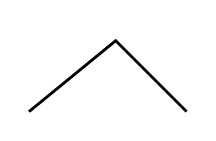
\begin{tikzpicture}[scale=1]
            \draw[-,line width=1pt] (0,0) -- (1.1,0.9) -- (2,0);
            \SetVertexSimple[Shape=circle,FillColor=white,MinSize=8 pt]
            \Vertex[x=0.00, y=0]{a}
            \Vertex[x=-0.5, y=1]{b}
            \Vertex[x=2., y=0]{c}
            \Edges(a,b,c)
            \tikzstyle{vertex}=[circle,minimum size=5pt]
            \node[vertex] (v0) at (1.1,0.9) {};
            \Edges(a,v0,c)
            
            %\node[vertex] (v1) at (-0.5,1) {b};
            %\node[vertex] (v2) at (2,0) {c};
            \end{tikzpicture} 
            \\
            &(a)&&(b)
        \end{tabular}
    \end{center}
    \caption{Dibujos de $K_3$} \label{fA4.1}
\end{figure}

Pero la definición es que un grafo es planar si se {\em puede} dibujar en el plano sin cruces de aristas, no si {\em todo} dibujo no tiene cruces. (Si la definición fuera así, ningún grafo seria planar, pues siempre se puede dibujar cualquier grafo con cruces). Otro ejemplo, ya visto, $K_4$ puede ser dibujado como en la Fig. \ref{fA4.2}-(a) y no parece planar, pero dibujado como en la Fig. \ref{fA4.2}-(b) muestra que $K_4$ es planar.

\begin{figure}[ht]
    \begin{center}
        \begin{tabular}{cccc}
            &
            \begin{tikzpicture}[scale=1]
            \SetVertexSimple[Shape=circle,FillColor=white,MinSize=8 pt]
            \Vertex[x=0.00, y=0]{a}
            \Vertex[x=2, y=0]{b}
            \Vertex[x=2, y=2]{c}
            \Vertex[x=0, y=2]{d}
            \Edges(a,b,c,d,a)
            \Edges(a,c)
            \Edges(b,d)
            \end{tikzpicture}
            &
            \qquad
            & 
            \begin{tikzpicture}[scale=1]
                    \SetVertexSimple[Shape=circle,FillColor=white,MinSize=8 pt]
            \Vertex[x=0.00, y=0]{a}
            \Vertex[x=1.15, y=2]{b}
            \Vertex[x=2.31, y=0]{c}
            \Vertex[x=1.15, y=0.8]{d}
            \Edges(a,b,c,d,a)
            \Edges(a,c)
            \Edges(b,d)
            \end{tikzpicture} 
            \\
            &(a)&&(b)
        \end{tabular}
    \end{center}
    \caption{Dibujos de $K_4$} \label{fA4.2}
\end{figure}

En vista de estos ejemplos, una pregunta es ¿existen grafos no planares? Por ejemplo si dibujáramos $K_{16}$ parecería imposible que fuera planar, dada la gran cantidad de cortes, pero ¿cómo podemos estar seguros?

Observemos primero que si $G$ es planar y $H$ es subgrafo de $G$, entonces $H$ es planar, pues, si podemos dibujar a $G$ en el plano sin cortes de aristas, entonces $H$ que esta ``metido'' en $G$, también puede ser así dibujado. Así, como ya vimos que $K_4$ es planar, sabemos que todo subgrafo de él es planar; es decir, todo grafo con cuatro o menos vértices es planar. Esta observación tiene consecuencias en la otra dirección también: si encontramos un grafo $H$ que {\em no} sea planar, entonces todo grafo $G$ que lo tenga como subgrafo deberá necesariamente ser no planar, pues si $G$ fuera planar, $H$ también lo seria. Así, si  queremos probar que $K_{16}$ no es planar, bastará con encontrar algún subgrafo mas sencillo de el que no lo sea. De hecho, probaremos que $K_5$ no es planar, con lo cual todos los grafos $K_n$, con $n\ge 5$ son no planares.

En lo que sigue veremos un arma poderosa para probar que un grafo es no planar: la llamada ``fórmula de Euler''.  \index{fórmula de Euler} Supongamos que un grafo {\em sí} es planar. Escojamos un diagrama
de él en el plano (puede haber muchos, escojamos uno). Este diagrama divide al plano en varias regiones. Por ejemplo, si $G$ esta representado por el dibujo de la Fig. \ref{fA4.3}, entonces se obtienen regiones que numeraremos como en la Fig. \ref{fA4.4} ($1$ es la región ``exterior'' a todo el grafo).

\begin{figure}[h]
    \begin{center}
        \begin{tikzpicture}[scale=0.7]
        \SetVertexSimple[Shape=circle,FillColor=white,MinSize=8 pt]
        \Vertex[x=0.00, y=0]{0}
        \Vertex[x=0.5, y=2]{1}
        \Vertex[x=0.8, y=-2]{2}
        \Vertex[x=1.5, y=-0.2]{3}
        \Vertex[x=1.8, y=-2.2]{4}
        \Vertex[x=3.5, y=1.9]{5}
        \Vertex[x=3, y=0.1]{6}
        \Vertex[x=3.7, y=-1.7]{7}
        \Vertex[x=4, y=-0.1]{8}
        \Vertex[x=6, y=0.3]{9}
        \Vertex[x=5.5, y=1.8]{10}
        \Vertex[x=6, y=-2.2]{11}
        \Vertex[x=6.8, y=2]{12}
        \Vertex[x=7, y=-1.8]{13}
        \Vertex[x=7.5, y=0.8]{14}
        \Vertex[x=8.5, y=1.8]{15}
        \Vertex[x=9, y=-1]{16}
        \Edges(0,1,3,4,2,0)
        \Edges(1,5,6,7,4,7,8,5,9,8,9,7,11,9,5,10,12,14,15,16,13,11)
        \end{tikzpicture} 
    \end{center}
\caption{Un grafo planar} \label{fA4.3}
\end{figure}

En realidad, también podríamos considerar a la región formada por las regiones $3$ y $4$ juntas, o $2$, $5$ y $6$ juntas, etc. Pero nuestra preocupación estará centrada en una de estas regiones ``simples'', a las cuales llamaremos {\em caras}.  \index{caras de un grafo planar}

\begin{figure}[h]
    \begin{center}
    \begin{tikzpicture}[scale=0.7]
    \SetVertexSimple[Shape=circle,FillColor=white,MinSize=8 pt]
    \Vertex[x=0.00, y=0]{0}
    \Vertex[x=0.5, y=2]{1}
    \Vertex[x=0.8, y=-2]{2}
    \Vertex[x=1.5, y=-0.2]{3}
    \Vertex[x=1.8, y=-2.2]{4}
    \Vertex[x=3.5, y=1.9]{5}
    \Vertex[x=3, y=0.1]{6}
    \Vertex[x=3.7, y=-1.7]{7}
    \Vertex[x=4, y=-0.1]{8}
    \Vertex[x=6, y=0.3]{9}
    \Vertex[x=5.5, y=1.8]{10}
    \Vertex[x=6, y=-2.2]{11}
    \Vertex[x=6.8, y=2]{12}
    \Vertex[x=7, y=-1.8]{13}
    \Vertex[x=7.5, y=0.8]{14}
    \Vertex[x=8.5, y=1.8]{15}
    \Vertex[x=9, y=-1]{16}
    \Edges(0,1,3,4,2,0)
    \Edges(1,5,6,7,4,7,8,5,9,8,9,7,11,9,5,10,12,14,15,16,13,11)
    \draw (-2, 1) node {1};
    \draw (3.5, 0) node {2};
    \draw (4.3, 0.8) node {3};
    \draw (4.3, -0.7) node {4};
    \draw (2.2, 0) node {5};
    \draw (0.8, 0) node {6};
    \draw (5.4, -1.2) node {7};
    \draw (7.2, -0.5) node {8};
    \end{tikzpicture} 
    \end{center}
    \caption{Regiones de un grafo planar} \label{fA4.4}
\end{figure}


Observemos que no podemos hablar propiamente de las caras del grafo (aunque a veces lo haremos así) pues ellas son en realidad dependientes del diagrama, no del grafo. Sin embargo, algo puede decirse acerca de ellas:

\begin{teorema}\label{tA4.1} (Fórmula de Euler) Sea $G$ un grafo conexo, con $v$ vértices, y $e$ aristas. Supongamos que en algún diagrama planar de $G$, existen $f$ caras. Entonces, $v-e+f=2$.
\end{teorema}

Antes de ver la prueba, observemos que, puesto que $v$ y $e$ dependen de $G$ y no del diagrama, la fórmula de Euler dice que no importa como dibujemos a $G$ en el plano (siempre y cuando esto sea posible), entonces siempre obtendremos $e-v+2$ caras. Por lo tanto, el \textit{número} de caras es algo independiente del
diagrama, y podemos hablar del ``número de caras de un grafo planar''. Otra observación es que en el número de caras estamos contando la cara infinita, es decir, la exterior a todo el grafo. Finalmente, observemos que se pide que $G$ sea conexo. La fórmula debe ser alterada en caso contrario.

\begin{proof}[Demostración del teorema \ref{tA4.1}] Supongamos que la fórmula de Euler no sea cierta. Es decir, supongamos que existen grafos planares para los cuales la fórmula no es válida. Tomemos, de todos estos contraejemplos, alguno con $e$ tan chico como sea posible, y llamemos $G$ a ese grafo. Observemos que $G$ debe tener por lo menos un ciclo, pues si fuera acíclico, como es conexo, sería un árbol. Ahora bien, en un árbol, $e=v-1$. Además, por ser acíclico, no hay caras, salvo la cara infinita, es decir, $f$ seria 1. Pero entonces $v-e+f=v-(v-1)+1=v-v+1+1=2$ y $G$ no sería un contraejemplo. Así pues, $G$ tiene al menos un ciclo. Sea $xy$ alguna arista perteneciente a algún ciclo, y consideremos $H=G-xy$. Como $xy$ pertenece a algún ciclo, es una arista que separa dos caras en $G$. Esas dos caras ahora son una sola en $H$. 
Ver Fig. \ref{fA4.5}.

\begin{figure}[ht]
    \begin{center}
    \begin{tabular}{cccc}
        &
        \begin{tikzpicture}[scale=0.7]
        \SetVertexSimple[Shape=circle,FillColor=white,MinSize=8 pt]
        \Vertex[x=0.00, y=0]{0}
        \Vertex[x=0.5, y=-1]{1}
        \Vertex[x=-0.5, y=-2]{2}
        \Vertex[x=0, y=-3]{3}
        \Vertex[x=2, y=-4]{4}
        \Vertex[x=3.5, y=-3]{5}
        \Vertex[x=3.5, y=-2]{6}
        \draw (3., -2.1) node {$y$};
        \Vertex[x=2, y=-1]{7}
        \draw (2, -1.5) node {$x$};
        \Vertex[x=1.8, y=0.2]{8}
        \Vertex[x=3, y=0]{9}
        \Vertex[x=5, y=-0.2]{10}
        \Vertex[x=4.5, y=-2.7]{11}
        \Edges(0,1,2,3,4,5,6)
        \Edges(6,7)
        \Edges(7,8,0)
        \Edges(1,7)
        \Edges(8,9,10,11,5)
        \draw (1.5, -2.5) node {$A$};
        \draw (3.5, -1) node {$B$};
        \end{tikzpicture}
        &
        \qquad
        & 
        \begin{tikzpicture}[scale=0.7]
        \SetVertexSimple[Shape=circle,FillColor=white,MinSize=8 pt]
        \Vertex[x=0.00, y=0]{0}
        \Vertex[x=0.5, y=-1]{1}
        \Vertex[x=-0.5, y=-2]{2}
        \Vertex[x=0, y=-3]{3}
        \Vertex[x=2, y=-4]{4}
        \Vertex[x=3.5, y=-3]{5}
        \Vertex[x=3.5, y=-2]{6}
        \draw (3., -2.1) node {$y$};
        \Vertex[x=2, y=-1]{7}
        \draw (2, -1.5) node {$x$};
        \Vertex[x=1.8, y=0.2]{8}
        \Vertex[x=3, y=0]{9}
        \Vertex[x=5, y=-0.2]{10}
        \Vertex[x=4.5, y=-2.7]{11}
        \Edges(0,1,2,3,4,5,6)
        \Edges(7,8,0)
        \Edges(1,7)
        \Edges(8,9,10,11,5)
        \end{tikzpicture} 
    \end{tabular}
\end{center}
    \caption{Eliminar una arista} \label{fA4.5}
\end{figure}
Así, si $f_H,e_H$ y $v_H$ denotan el número de caras, aristas y vértices de $H$ respectivamente, te\-ne\-mos que $f_H=f-1$. Además, como borramos una arista, $e_H=e-1$, y como el número de vértices no cambia, $v_H=v$.

Pero, $e_H=e-1$ es menor que $e$, y $G$ era un contraejemplo con un número tan chico como fuera posible de aristas, por lo tanto, $H$ no es un contraejemplo, es decir, $v_H-e_H+f_H=2$. Reemplazando, obtenemos:
$$
v-e+f=v_H-(e_H+1)+f_H+1=v_H-e_H-1+f_H+1=v_H-e_H+f_H=2,
$$
lo cual dice que $G$ no es un contraejemplo, absurdo.
\end{proof}

La fórmula de Euler es una herramienta muy poderosa en la teoría de grafos planares. Para empezar, permite probar que un grafo planar no puede tener muchas aristas, en relación a sus vértices 
\begin{corolario}\label{cA4.1} Sea $G$ un grafo planar con al menos $3$ vértices. Entonces, $e\le 3v-6$, donde $e$ es el número de aristas y $v$ el número de vértices de $G$.
\end{corolario} \begin{proof} Consideremos las caras de $G$. Si es una cara distinta de la cara infinita, es porque viene de un ciclo. Ahora bien, todo ciclo debe tener por lo menos $3$ aristas, así que podemos concluir que hay por lo menos $3$ aristas en el borde de esa cara. Si, en cambio, es la cara infinita y el grafo tiene más de tres aristas entonces ``toca'' $3$ o más aristas. Si el grafo tiene menos de $3$ aristas (y ningún ciclo), es uno de los de la Fig. \ref{fA4.6}.  Como estamos suponiendo que hay al menos $3$ vértices, en realidad solo hay que considerar el último caso, y ese tiene $e=2$, $v=3$, y $2\le 3 \cdot 3-6$.

    \begin{figure}[ht]
        \begin{center}
        \begin{tabular}{cccc}
            &
            \begin{tikzpicture}[scale=0.7]
            \SetVertexSimple[Shape=circle,FillColor=white,MinSize=8 pt]
            \Vertex[x=0.00, y=0]{0}
            \Vertex[x=2, y=0]{1}
            \Edges(0,1)
            \end{tikzpicture}
            &
            \qquad\qquad
            & 
            \begin{tikzpicture}[scale=0.7]
            \SetVertexSimple[Shape=circle,FillColor=white,MinSize=8 pt]
            \Vertex[x=0.00, y=0]{0}
            \Vertex[x=2, y=0]{1}
            \Vertex[x=4, y=0]{2}
            \Edges(0,1,2)
            \end{tikzpicture} 
        \end{tabular}
    \end{center}
        \caption{Grafos acíclicos con menos de 3 aristas} \label{fA4.6}
    \end{figure}
    
Así pues, podemos suponer que en nuestro grafo, todas las caras tienen al menos $3$ aristas en su borde. Es decir:
$$
\begin{aligned}
3\le &\,\text{ Número de aristas en el borde de cara }1 \\
3\le &\,\text{ Número de aristas en el borde de cara }2\\
&\vdots \\
3\le &\,\text{ Número de aristas en el borde de cara }f.
\end{aligned}
$$
Si sumamos estas desigualdades, del lado izquierdo obtendremos $3f$. En el lado derecho, cada arista puede, o bordear dos caras, o bordear una. Pero ciertamente, no puede haber aristas que sean borde de $3$ caras. Así, si sumamos en el lado izquierdo, la suma nos dará menor o igual a $2e$. Por lo tanto, $3f\le 2e$. Tomando la fórmula de Euler y multiplicándola por $3$, obtenemos: $3v-3e+3f=6$. Usando ahora $3f\le 2e$, tenemos
$$
6=3v-3e+3f\le 3v-3e+2e=3v-e,$$ es decir, $e\le 3v-6$.
\end{proof}

Este corolario nos permite probar inmediatamente la no planaridad de un número significativo de grafos. Por ejemplo, recordemos que queríamos ver que $K_5$ era no planar. Esto lo obtenemos en forma directa, pues $K_5$ tiene $5$ vértices y $10$ aristas, por lo tanto, si fuera planar debiéramos tener que $10\le 3\cdot  -6=15-6=9$, lo cual no es cierto.
\end{section}

\begin{section}{El problema del agua-luz-gas}\label{Ap4.2} Este es un conocido problema de escuela primaria: existen tres casas, y tres centrales: la del agua, la de la luz y la del gas. Trazar las cañerías desde las centrales a las casas sin que se crucen. Una solución (pero haciendo trampa) es mandar las tres cañerías a una casa, y de ella sacarlas las tres a la otra, y de ella las tres a la otra:

    \tikzstyle{startstop} = [rectangle, rounded corners, minimum width=3cm, minimum height=1cm,text centered, draw=black, fill=gray!30]
    \tikzstyle{servicio} = [rectangle, rounded corners, minimum width=1cm, minimum height=1cm,text centered, draw=black, fill=gray!30]
 
\begin{figure}[ht]
    \begin{center}
        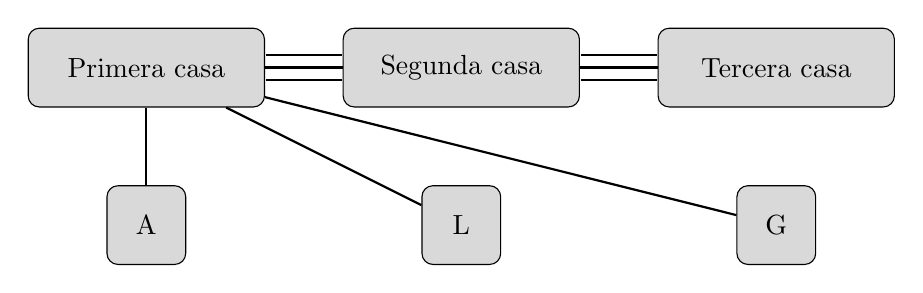
\begin{tikzpicture}[node distance=2cm,scale=0.8]
            \node (casa1) [startstop] {Primera casa};
            \node (casa2) [startstop, xshift=4cm] {Segunda casa};
            \node (casa3) [startstop, xshift=8cm] {Tercera casa};
            \node (A) [servicio, below of=casa1] {A};
            \node (L) [servicio, below of=casa2] {L};
            \node (G) [servicio, below of=casa3] {G};
            \draw [thick,-,>=stealth] (A) -- (casa1);
            \draw [thick,-,>=stealth] (L) -- (casa1);
            \draw [thick,-,>=stealth] (G) -- (casa1);
            \draw [thick,-,>=stealth] (casa1) -- (casa2);
            \draw [thick,-,>=stealth] (1.9,0.2) -- (3.1,0.2);
            \draw [thick,-,>=stealth] (1.9,-0.2) -- (3.1,-0.2); 
            \draw [thick,-,>=stealth] (casa2) -- (casa3);
            \draw [thick,-,>=stealth] (6.9,0.2) -- (8.1,0.2);
            \draw [thick,-,>=stealth] (6.9,-0.2) -- (8.1,-0.2); 
        \end{tikzpicture}
    \end{center}
    \caption{Una solución tramposa} \label{fA4.7}
\end{figure}

En realidad, no permitiremos el uso de intermediarios, es decir el problema será llevar directamente la cañería desde cada central a cada casa. En el lenguaje de la teoría de grafos, consiste en representar, en el plano, al grafo $K_{3,3}$ Fig. \ref{fA4.8}.

\begin{figure}[ht]
    \begin{center}
        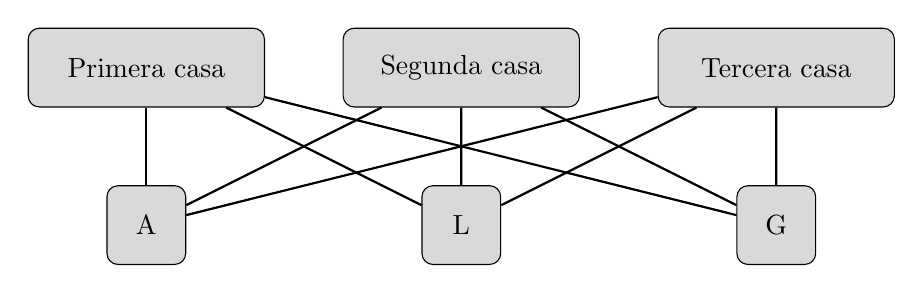
\begin{tikzpicture}[node distance=2cm,scale=0.8]
            \node (casa1) [startstop] {Primera casa};
            \node (casa2) [startstop, xshift=4cm] {Segunda casa};
            \node (casa3) [startstop, xshift=8cm] {Tercera casa};
            \node (A) [servicio, below of=casa1] {A};
            \node (L) [servicio, below of=casa2] {L};
            \node (G) [servicio, below of=casa3] {G};
            \draw [thick,-,>=stealth] (A) -- (casa1);
            \draw [thick,-,>=stealth] (L) -- (casa1);
            \draw [thick,-,>=stealth] (G) -- (casa1);
            \draw [thick,-,>=stealth] (A) -- (casa2);
            \draw [thick,-,>=stealth] (L) -- (casa2);
            \draw [thick,-,>=stealth] (G) -- (casa2);
            \draw [thick,-,>=stealth] (A) -- (casa3);
            \draw [thick,-,>=stealth] (L) -- (casa3);
            \draw [thick,-,>=stealth] (G) -- (casa3);
        \end{tikzpicture}
    \end{center}
    \caption{Luz-agua-gas es $K_{3,3}$} \label{fA4.8}
\end{figure}

La pregunta es entonces si $K_{3,3}$ es planar o no. Veamos si podemos usar esta fórmula que probamos recién: $K_{3,3}$ tiene $9$ aristas, y $6$ vértices. Desafortunadamente, $3 \cdot 6-6=18-6=12$ es ciertamente mayor que $9$, así que solo sabemos que quizás es planar. Pero, observemos que $K_{3,3}$, por ser bipartito, no tiene ningún triángulo como subgrafo. Así pues, deduciremos la no planaridad de $K_{3,3}$ del si\-guien\-te

\begin{corolario}\label{cA4.2} Si $G$ es un grafo planar con por lo menos $3$ vértices y que no tiene ningún triángulo como subgrafo, entonces $e\le 2v-4$.
\end{corolario}
\begin{proof} Es similar a la demostración del corolario \ref{cA4.1}, pero como no hay triángulos, todo ciclo tiene por lo menos $4$ aristas, es decir, cada cara esta bordeada por al menos $4$ aristas. Las únicas
excepciones con al menos $3$ vértices son los de la fig. \ref{fA4.9}

\begin{figure}[ht]
    \begin{center}
    \begin{tabular}{cccccc}
    &
    \begin{tikzpicture}[scale=0.5]
    \SetVertexSimple[Shape=circle,FillColor=white,MinSize=8 pt]
    \Vertex[x=0.00, y=0]{0}
    \Vertex[x=2, y=0]{1}
    \Vertex[x=4, y=0]{2}
    \Edges(0,1,2)
    \end{tikzpicture}
    &
    \qquad
    & 
    \begin{tikzpicture}[scale=0.5]
    \SetVertexSimple[Shape=circle,FillColor=white,MinSize=8 pt]
    \Vertex[x=0.00, y=0]{0}
    \Vertex[x=2, y=0]{1}
    \Vertex[x=4, y=0]{2}
    \Vertex[x=6, y=0]{3}
    \Edges(0,1,2,3)
    \end{tikzpicture} 
    &
    \qquad
    &
    \begin{tikzpicture}[scale=0.5]
    \SetVertexSimple[Shape=circle,FillColor=white,MinSize=8 pt]
    \Vertex[x=0.00, y=0]{0}
    \Vertex[x=0, y=1.3]{1}
    \Vertex[x=-1, y=-1]{2}
    \Vertex[x=1, y=-1]{3}
    \Edges(0,1,0,2,0,3)
    \end{tikzpicture} 
    \end{tabular}
\end{center}
    \caption{Grafos acíclicos con menos de $4$ aristas y al menos $3$
    vértices} \label{fA4.9}
\end{figure}

En el primer caso, $e=2$, $v=3$ y $2 \cdot 3-4=6-4=2$. En el segundo y terceros, $e=3$, $v=4$ y $2 \cdot 4-4=8-4=4\ge 3$. Así pues, podemos suponer que cada cara esta bordeada por al menos $4$ aristas. Sumando cara a cara, como antes, obtenemos ahora $4f\le 2e$, es decir, $2f\le e$. Multiplicando la fórmula de Euler por $2$, tenemos: $4=2v-2e+2f\le 2v-2e+e=2v-e$, es decir, $e\le 2v-4$.
\end{proof}

Retornando a $K_{3,3}$, como no tiene triángulos, podemos aplicar este corolario, y si fuera planar, debería cumplirlo. Pero habíamos dicho que $K_{3,3}$ tiene $9$ aristas y $6$ vértices, y $2\cdot 6-4=12-4=8$. Por lo tanto, $K_{3,3}$ no es planar.

Una ultima observación acerca de grafos planares: existe un teorema muy interesante, de difícil demostración (la prueba tiene $31$ casos y subcasos para considerar) debido a Kuratowski, que  \index{Teorema de Kuratowski}  dice que $K_5$ y $K_{3,3}$ son los dos grafos ``básicos'' no planares, en el siguiente sentido: un grafo $G$ es no planar si y solo si existe un subgrafo de $G$, digamos $H$, tal que $H$ se ``ve'' como $K_5$ o como $K_{3,3}$, es decir, $H$ es uno de ellos, excepto que tal vez, ``agregue'' en alguna o algunas
aristas, vértices en el medio. Por ejemplo, $H$ puede lucir como en la fig. \ref{fA4.10}.

\begin{figure}[ht]
    \begin{center}
    \begin{tikzpicture}[scale=1]
    \SetVertexSimple[Shape=circle,MinSize=5 pt,FillColor=white]
    \Vertex[x=0.00, y=2.00]{1}
    \Vertex[x=1.90, y=0.62]{2}
    \Vertex[x=1.18, y=-1.62]{3}
    \Vertex[x=-1.18, y=-1.62]{4}
    \Vertex[x=-1.90, y=0.62]{5}
    \Edges(1,2,3,4,5,1)
    \Edges(1,3,5,2,4,1)
    \Vertex[x=0.95, y=1.31]{a}
    \Vertex[x=0.3, y=1.08]{b}
    \Vertex[x=1.54, y=-0.5]{c}
    \Vertex[x=-0.36, y=-0.5]{d}
    \Vertex[x=-0.95, y=1.31]{e}
    \Vertex[x=-0.39, y=-1.62]{f}
    \Vertex[x=0.39, y=-1.62]{g}
    \end{tikzpicture}
    \end{center}
    \caption{Un grafo no planar ``básico''}\label{fA4.10}
\end{figure}

\end{section}


\begin{section}{El teorema de los cuatro colores} \label{Ap4.3}

Juntaremos ahora lo que hemos visto en esta sección con lo que vimos en la anterior, para tratar uno de los problemas mas famosos y recalcitrantes de la teoría de grafos, a saber: ¿cuántos colores se necesitan para colorear un grafo planar? En otras palabras, si quiero estar seguro de poder colorear propiamente los vértices de cualquier grafo planar, ¿cuántos colores necesito tener? De hecho, una pregunta más básica sería si existe una cantidad finita de colores que me permitan colorear cualquier tipo de grafo planar, por grande que sea. (Es claro que la respuesta para grafos en general es negativa, pues $K_n$ requiere $n$ colores.) Como $K_4$ es planar, sabemos que necesitamos por lo menos $4$ colores. No podemos decir que necesitamos necesariamente $5$, pues hemos visto que $K_5$ no es planar. Pero, podría haber otro grafo, complicado pero planar, que requiera $5$, o más, colores. A mediados del siglo pasado la conjetura de que bastan $4$ colores fue hecha, y en $1\,879$ A. Kempe publicó una prueba de este hecho, que paso a llamarse el teorema de los cuatro colores. Desafortunadamente para Kempe, en $1\,889$ (diez años después) otro matemático, P. Heawood, probó que la prueba de Kempe contenía un error. Heawood no fue completamente destructivo: mostró que adaptando la prueba de Kempe, podía probarse que con $5$ colores bastaba para colorear cualquier grafo planar (el teorema de los cinco colores). Así pues, quedo planteado el problema de saber si el teorema de los cuatro colores era cierto, o bien si existía algún grafo planar para el cual $5$ colores fueran necesarios. (Pero, al menos, gracias a Heawood, no era necesario buscar alguno que necesitara $6$, o $7$ u $8$ colores, pues no existen, gracias al teorema de los cinco colores.) De hecho, en ese mismo artículo, Heawood probó más cosas: definió el \textit{género de un grafo}, que es un número entero no negativo, y que no daremos aquí su definición. Heawood demostró que existía una \index{género de un grafo} fórmula (expresión aritmética) que para cada género $g\ge 1$ da la cantidad de colores que permite colorear todos los grafos de género $g$. Los grafos planares tiene género igual a $0$ y aplicando la fórmula para $g=0$ obtenemos el número $4$. Sin embargo, Heawood pudo probar que la fórmula es válida si $g$ es mayor o igual a 1. El hecho de que esta fórmula existiera ``convenció'' a mucha gente de que el teorema de los cuatro colores debía ser cierto y que una prueba no tardaría en hallarse. Sin embargo, pese al esfuerzo de muchos matemáticos y pese al desarrollo de la teoría, el teorema de los cuatro colores no pudo probarse hasta $1975$, cuando dos matemáticos \index{Teorema de los cuatro colores} norteamericanos, K. Appel y W. Haken, lo probaron. Más aún, no pudieron probarlos solos, sino que debieron usar la ``ayuda'' de una poderosa (para esa época) computadora. Así, aún cuando el teorema fue probado, un gran sentimiento de desconfianza se generó, sobretodo en una época en la cual el acceso fácil a tiempo de computadora no era común. Decenas de años han pasado y la prueba ahora ha sido controlada numerosas veces y no genera tanta resistencia como antes. Aún así, si alguien pudiese publicar una prueba que fuese ``leíble por humanos'' sería muy bien bienvenido.

Obviamente por lo dicho arriba, no daremos una prueba del teorema de los cuatro colores. Sí daremos una del teorema de los cinco colores\index{Teorema de los cinco colores}, mencionando donde se encuentra la dificultad de la demostración del teorema de los  cuatro colores, y dando una idea de que es lo que Appel y Haken (y el computador) hicieron. 

\begin{lema} \label{lA4.3.1} Sea $G$ un grafo planar. Entonces, existe un vértice de $G$ de valencia $5$ o menos.
\end{lema}
\begin{proof} Si el orden de $G$ es menor o igual a $2$, esto es obvio, pues la valencia de cualquier vértice no superará $2$. Así, podemos suponer que hay al menos $3$ vértices, y por lo tanto, sabemos que $e\le 3v-6$, donde $e$ es el numero de aristas y $v$ el de vértices.

Supongamos ahora que la valencia de todos los vértices sea al menos $6$. Entonces, si sumamos las valencias de todos los vértices, la suma sera mayor o igual a $6v$. Pero la suma de todos las
valencias es igual a $2e$ (lema del apretón de manos). Así, tenemos que $2e\ge 6v$. Por otro lado, como $e\le 3v-6$, tenemos que $2e\le 6v-12$, es decir, obtenemos $6v-12\ge 2e\ge 6v$, o $-12\ge 0$, lo cual es un absurdo.
\end{proof}

\begin{teorema}\label{tA4.3.1}(Teorema de los cinco colores) Si $G$ es planar, $\chi (G)\le 5$.
\end{teorema}
\begin{proof}
 Supongamos que no sea cierto. De todos los contraejemplos al teorema, escojamos uno con la menor cantidad de
vértices posible y llamémosle $G$. Por el lema anterior, existe un vértice $x$ de $G$ con valencia menor o igual a 5. Consideremos $H=G-\{x\}$, que es un grafo con menos vértices que $G$ y por lo tanto no puede ser un contraejemplo; es decir, $\chi (H)\le 5$. Así, podemos colorear $H$ con 5 colores. Si la valencia de $x$ en $G$ es $0,1,2,3$ o $4$, los vértices adyacentes a $x$ ``usan'' a lo sumo $4$ de los $5$ colores, así que podemos colorear a $x$ con el quinto color, y tendríamos que $\chi (G)=5$, lo cual no es posible pues $G$ es un contraejemplo. Así pues, podemos suponer que la valencia de $x$ es $5$. Ahora bien, si los cinco vértices adyacentes a $x$ no usan cinco colores, estamos como antes, y podemos colorear a $x$ con el color faltante. Así, no solo podemos suponer que hay cinco vértices adyacentes a $x$, sino también que cada uno esta coloreado con un color distinto. Llamemos a estos vértices $y,z,u,w,t$, y supongamos que $y$ de color $1$, $z$ de color $2$, etc.

\begin{figure}[h]
    \begin{center}
\begin{tikzpicture}[scale=0.6,]
%\SetVertexSimple[Shape=circle,FillColor=white,MinSize=8 pt]
\Vertex[x=0.00, y=0, L=$0$]{0}
\Vertex[x=0.5, y=2, L=$1$]{1}
\Vertex[x=4, y=1.5, L=$2$]{2}
\Vertex[x=3, y=-1.4, L=$3$]{3}
\Vertex[x=0.5, y=-2, L=$4$]{4}
\Vertex[x=-3, y=0, L=$5$]{5}
\draw (-0.9, 0.6) node {$x$};
\draw (-0.6, 2) node {$y$};
\draw (2.9, 1.7) node {$z$};
\draw (2.0, -1.6) node {$u$};
\draw (-0.7, -2) node {$w$};
\draw (-3.9,0.5) node {$t$};
\Edges(0,1,0,2,0,3,0,4,0,5)
\end{tikzpicture} 
\end{center}
\caption{$x$ es un vértice de valencia $5$ en el grafo planar.}\label{fA4.11}
\end{figure}

Supongamos primero que no haya, entre $y$ y $u$, ningún camino tal que el color de todos sus vértices sea $1$ o $3$. Entonces, podemos cambiarle el color a $y$, de color $1$ a color $3$. Además, a los vértices adyacentes a $y$ que tengan color $3$, les cambiamos el color de $3$ a $1$. A los vértices adyacentes a estos, que tengan color $1$, los cambiamos a $3$, y así sucesivamente. Después de realizar todos estos cambios, todavía tenemos un coloreo propio. Ahora bien, como estamos suponiendo que no hay ningún camino de
color $1$ y $3$ exclusivamente entre $y$ y $u$, resulta que $u$ no cambia de color, es decir, retiene el color $3$. Pero $y$ ahora tiene también el color $3$, y ningún otro vértice adyacente a $x$ tiene el color $1$. Pero, entonces, podemos colorear a $x$ con el color $1$ sin problemas, absurdo pues $\chi(G)\ge 6$.

Así pues, existe un camino con todos los vértices de color $1$ y $3$ entre $y$ y $u$. Igualmente, si no hubiera ningún camino con todos los vértices de color $2$ y $4$ entre $z$ y $w$, le podemos cambiar el color a $z$ de $2$ a $4$ sin problemas, y colorear a $x$ con el color $2$. Así, también podemos suponer que existe un camino con todos los vértices de color $2$ y $4$ entre $z$ y $w$. 

\begin{figure}[h]
    \begin{center}
    \begin{tikzpicture}[scale=0.6]
    \draw[-,line width=1pt,dashed] (0.5,2) -- (2.5,3)-- (5,2.5) -- (5.5,1)-- (5.5,0.2) -- (3, -1.4) ;
    \draw[-,line width=1pt,dashed] (4,1.5) -- (6,0.5) -- (6.5,-0.5)-- (5.5,-2.3) --(3,-2.8) -- (0.5, -2) ;
    \SetVertexSimple[Shape=circle,FillColor=white,MinSize=8 pt]
    \Vertex[x=0.00, y=0]{0}
    \Vertex[x=0.5, y=2]{1}
    \Vertex[x=4, y=1.5]{2}
    \Vertex[x=3, y=-1.4]{3}
    \Vertex[x=0.5, y=-2]{4}
    \Vertex[x=-3, y=0]{5}
    \draw (-0.5, 0.4) node {$x$};
    \draw (-0.1, 2) node {$y$};
    \draw (3.4, 1.7) node {$z$};
    \draw (2.4, -1.6) node {$u$};
    \draw (-0.2, -2) node {$w$};
    \draw (-3.4,0.5) node {$t$};
    \Edges(0,1,0,2,0,3,0,4,0,5)
    \end{tikzpicture} 
    \end{center}
    \caption{Caminos de $y$ a $u$ y de $z$ a $w$} \label{fA4.12}
\end{figure}


Por la Fig. \ref{fA4.12} es claro que tenemos un problema: ¿por donde se cruzan los caminos $A$ y $ B$? Más precisamente, el camino $A$, junto con las aristas $xy$ y $xu$, forma un ciclo $C$. Este ciclo tiene un interior y un exterior. El ciclo $ D$ formado por $B$ y las aristas $xz$, $xw$ cruza al ciclo $C$ en el punto
$x$, pues la arista $xz$ esta en el interior y la arista $xw$ en el exterior de $C$. Por lo tanto, $D$ debe cruzar a $C$ en algún otro punto. Pero no puede hacerlo, pues en el resto, $C$ esta coloreado con los colores $1$ y $3$, y $D$ con los colores $2$ y $4$. Hemos llegado a una contradicción.
\end{proof}

Analicemos un poco la prueba: hemos probado dos cosas. La primera es que todo grafo planar debe tener una de las siguientes ``configuraciones'', es decir, parte de él debe lucir como alguno de los grafos de la Fig. \ref{fA4.13}.

\begin{figure}[h]
    \begin{center}
    \begin{tikzpicture}[scale=0.5]
    \SetVertexSimple[Shape=circle,FillColor=white,MinSize=8 pt]
    \Vertex[x=0.00, y=0]{0}
    \Vertex[x=3, y=0]{1}
    \Vertex[x=5, y=0]{2}
    \Vertex[x=7, y=1]{3}
    \Vertex[x=9, y=-1]{4}
    \Vertex[x=11, y=1]{5}
    \Vertex[x=13, y=1]{6}
    \Vertex[x=15, y=-1]{7}
    \Vertex[x=17, y=1]{8}
    \Vertex[x=15, y=-3]{9}
    \Edges(1,2)
    \Edges(3,4,5)
    \Edges(6,7,8,7,9)
    \Vertex[x=0, y=-3]{a}
    \Vertex[x=4, y=-3]{b}
    \Vertex[x=0, y=-7]{c}
    \Vertex[x=4, y=-7]{d}
    \Edges(a,d)
    \Edges(b,c)
    \Vertex[x=2, y=-5]{e}
    \Vertex[x=7, y=-4]{f}
    \Vertex[x=11, y=-4]{g}
    \Vertex[x=9, y=-5.5]{h}
    \Vertex[x=9, y=-3]{i}
    \Vertex[x=7, y=-7]{j}
    \Vertex[x=11, y=-7]{k}
    \Edges(f,h,g,h,i,h,j,h,k)
    \end{tikzpicture} 
    \end{center}
\caption{Posibles configuraciones} \label{fA4.13}
\end{figure}

Esto lo probamos con el lema \ref{lA4.3.1}. Es decir, probamos que ese conjunto de configuraciones es lo que se llama \textit{inevitable}.

Además, en segunda instancia, probamos que si un grafo planar tiene una de esas configuraciones, puede ser coloreado con $5$ colores (esto es lo que hicimos en el teorema). Es decir, probamos que ese conjunto de con\-fi\-gu\-ra\-cio\-nes es lo que se llama \textit{irreducible} (para $5$ colores). 

Kempe creyó que había sido capaz de probar que todo grafo planar que tuviera esas configuraciones podía ser coloreado con $4$ colores, y muchos autores después de Heawood trataron de probar lo mismo. Pero luego se descubrieron nuevas técnicas, tanto para probar que un conjunto de configuraciones es irreducible, como para probar que es inevitable. Lo que no se podía hacer era encontrar un conjunto que fuera al mismo tiempo irre\-du\-ci\-ble (para $4$ colores) e inevitable. Finalmente, Appel y Haken encontraron un conjunto que satisfacía esas propiedades. Solo que en vez detener $6$ elementos, como en el caso del teorema de $5$ colores, el conjunto de Appel y Haken tiene $1\,480$ elementos, y ningún ser humano es capaz de probarlo, sino que es necesario un computador para comprobar la inevitabilidad e irreducibilidad.

El problema con la prueba de  Appel y Haken es que se basa en programas de computadora y entonces uno debe confiar en que no hay errores de programación. Incluso algunos matemáticos han dicho que la prueba contiene varios errores, pero  no han podido mostrarlos fehacientemente. 

En  cierta manera esta polémica si diluyó en el año 2005 cuando Benjamin Werner y Georges Gonthier formalizaron una prueba del teorema con el asistente de pruebas Coq. Esto eliminó la necesidad de confiar en los diversos programas informáticos utilizados para verificar casos particulares; solo es necesario confiar en el kernel de Coq, construido alrededor de un núcleo bien delimitado, el cual la comunidad científica considera que no debe tener errores. A esta altura está claro que esta prueba es mucho más confiable que la demostración de muchos teoremas importantes de la matemática de cientos de páginas propensos a errores humanos.

La prueba con Coq se encuentra en el artículo de G. Gonthier ``Formal Proof—The Four-Color Theorem'', Notices of the American Mathematical Society, 55 (11): 1382–1393, MR 2463991 (2008).  

\end{section}
